Ce projet d'application s'inscrivant dans un travail de groupe, nous avons, dès la conception de l'application, puis lors de son développement, attaché une grande importance à l'organisation et à la répartition des tâches.

\section{Gestionnaire de version Git}
D'un point de vue technique, cette préoccupation d'organisation s'est traduite par l'utilisation du gestionnaire de versions Git, non seulement afin de générer des copies de sauvegarde de notre code source, mais également pour pouvoir travailler en parallèle les uns des autres grâce au système de branches.

L'utilisation de cet outil nous a été d'une grande utilité, notamment lors de la répartition des tâches en nous permettant de gérer indépendamment les différentes parties de l'application.

\section{Organisation modulaire}
Toujours dans l'optique d'une répartition simple et non ambiguë du travail à accomplir, nous avons essayé de rendre le développement de l'application le plus modulaire possible. Ainsi, nous avons séparé au maximum les modules liés à la gestion du rendu 3D des modules liés au calcul des solutions.

Enfin, dans le but d'unifier notre code source, nous avons établi des conventions communes quant à la nomenclature des variables et des fonctions.

Finalement voici le diagramme de Gantt de notre projet :

\begin{figure}[h]
 \centering
 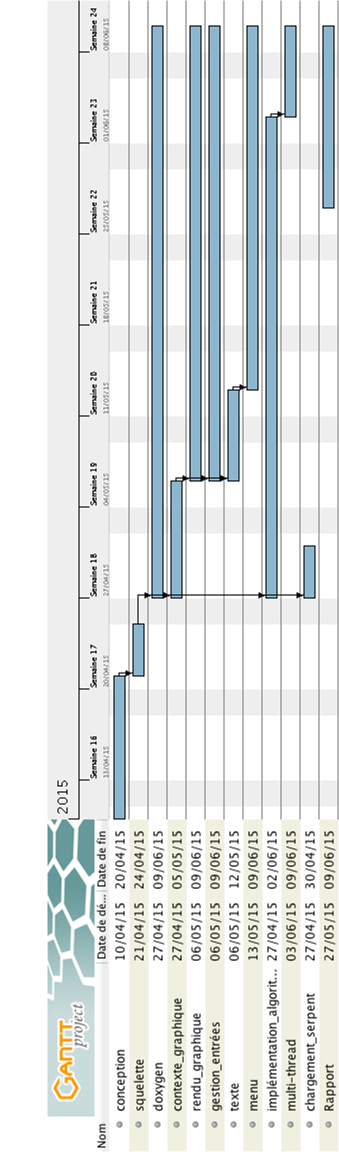
\includegraphics[scale=0.5,keepaspectratio=true]{img/gantt.png}
 \caption{Diagramme de Gantt}
 \label{Gantt}
\end{figure}